% -*- root: ../lsnotess.tex -*-

\chapter{Discrete-time Linear Time-Invariant systems}

% % \begin{chapquote}{Author's name, \textit{Source of this quote}}
% % ``This is a quote and I don't know who said this.''
% % \end{chapquote}

% We will encounter several types of signals in our study of linear systems. This chapter discusses the different signals we will be used at some point during our discussion of linear systems. In this chapter we will cover both continuous-time and discrete-time signals; in fact this will be our general approach in all chapter, where we will cover both continuous-time and discrete-time concepts. 

% \section{Exponential Signals}
% \subsection{Continuos-time real exponential}
% A continuous-time real exponential signal is represented as the following,
% \[ x\left(t\right) = ae^{bt}, \,\,\, a, b \in \mb{R} \]
% \noindent where, $t$ is time, $a$ is the amplitude of the signal when $t = 0$, and $b$ the parameter indicate whether the $x\left(t\right)$ is an exponentially growing signal $\left(b > 0\right)$ or a exponentially decaying signal $\left(b < 0\right)$. 
% \begin{figure}[h]
% \centering
%     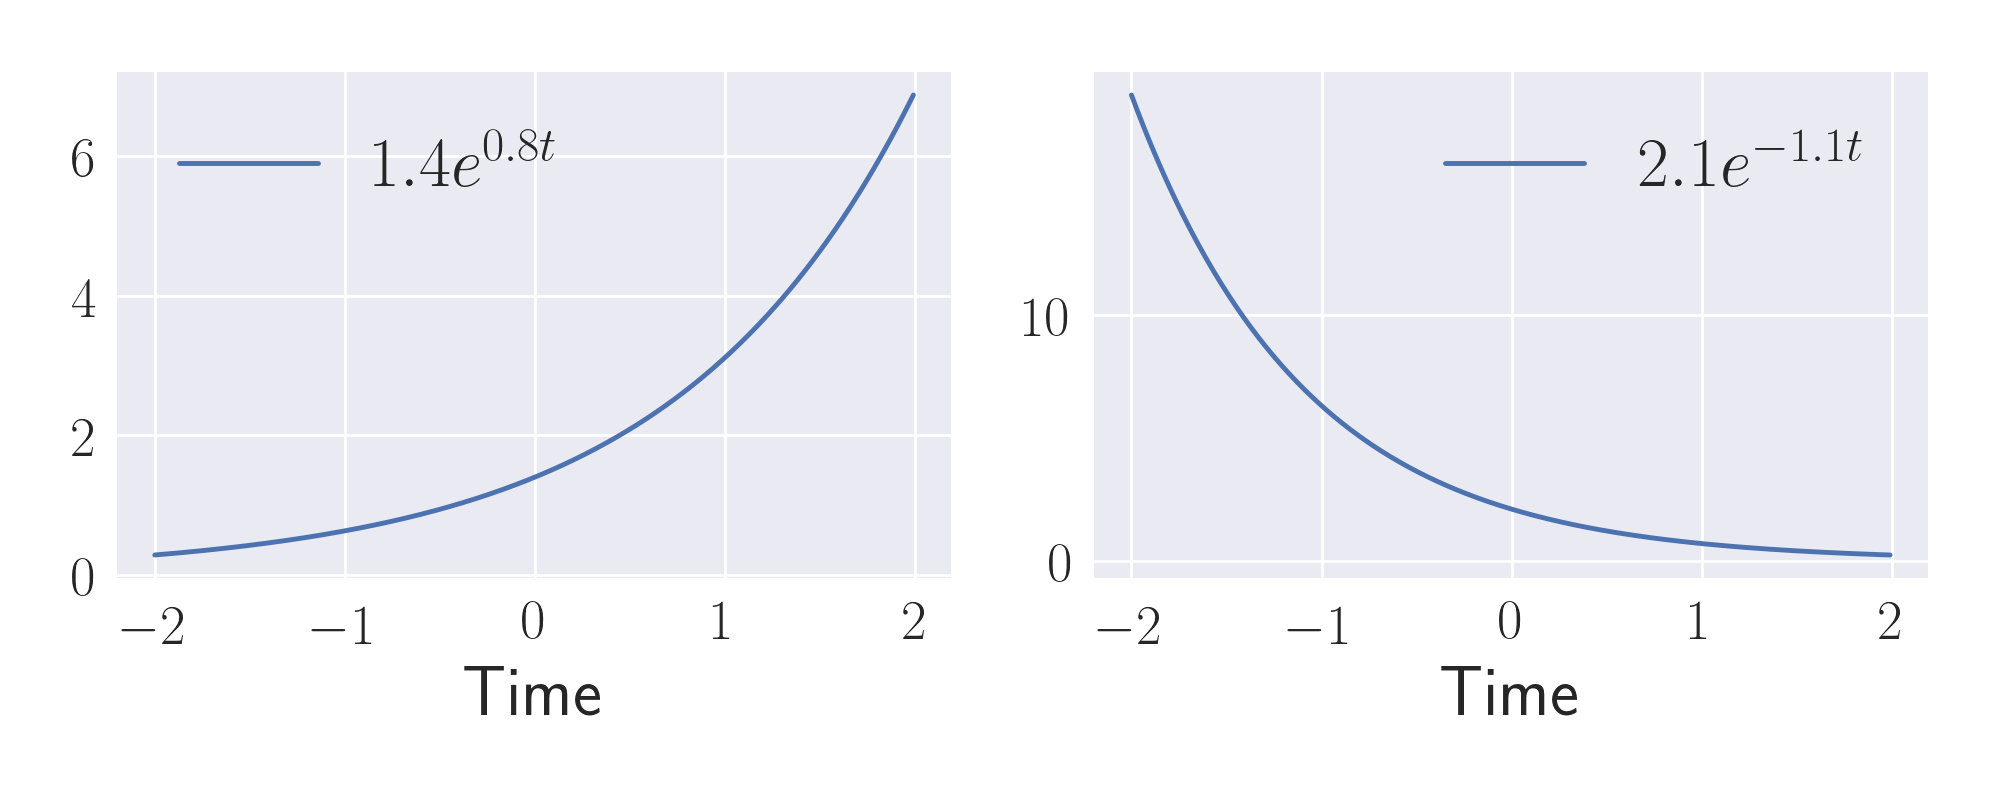
\includegraphics[width=0.95\textwidth]{figs/ch2-expsig.png}
% \caption{Continuous-time real exponential signals -- growing exponential on the left and a decaying exponential on the right.} \label{fig:ch2-expsig}
% \end{figure}
% When $b = 0$, then we get a constant signal $x\left(t\right) = a, \,\, \forall t$. The plot of $x\left(t\right)$ for different values of b is given in Fig. \ref{fig:ch2-expsig}.

% Exponential signals are often observed in physical systems. They play an important role in the analysis of linear time-invariant system. 

% \subsection{Discrete-time real exponential}
% A discrete-time real exponential signal is represented as,
% \[ x\dt{n} = b \times a^n, \quad \quad a, b \in \mb{R} \text{ and } n \in \mb{Z} \]
% This signal represents a growing exponential if $a > 1$, and its a decaying exponential if $0 < a < 1$; these are shown in Fig \ref{fig:ch2_discexpsig}. 

% \begin{figure}[h]
% \centering
%     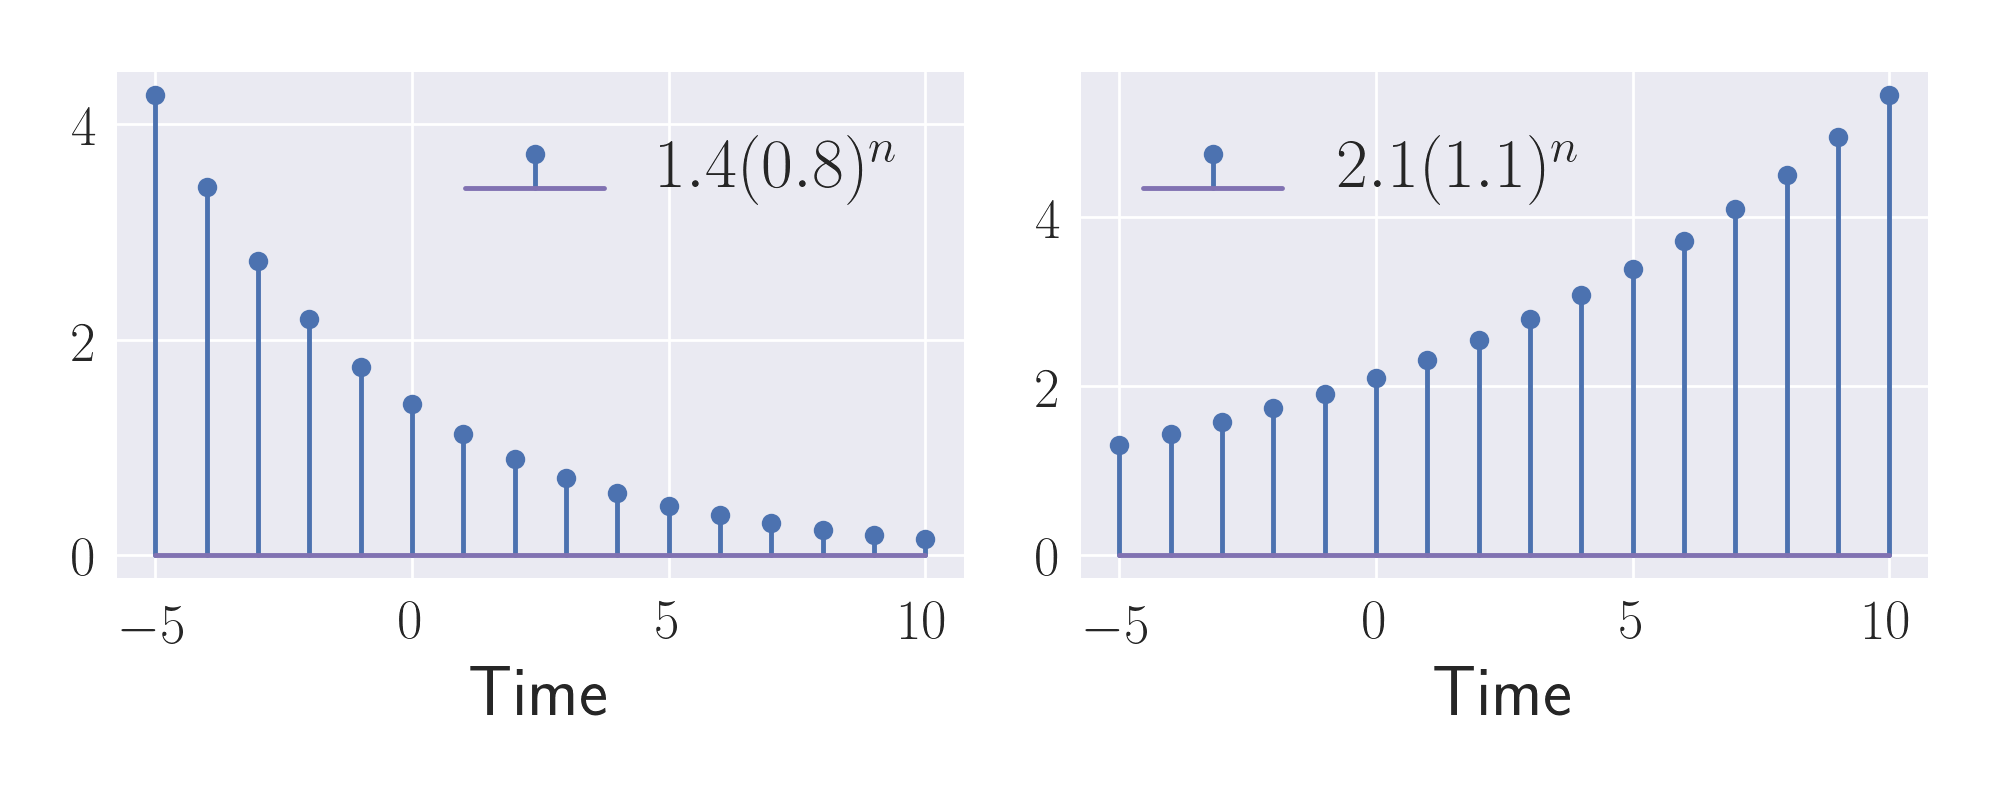
\includegraphics[width=0.95\textwidth]{figs/ch2-discexpsig.png}
% \caption{Continuous-time real exponential signals -- growing exponential on the left and a decaying exponential on the right.} \label{fig:ch2_discexpsig}
% \end{figure}

% \begin{problem*}[frametitle=Discrete-time exponential signals]
%     \begin{enumerate}
%         \item What does $a^n$ look like when: (a) $-1 < a < 0$; and (b) $a < -1$?
%     \end{enumerate}
% \end{problem*}

% \section{Sinusoidal Signals}
% \subsection{Continuous-time sinusoids}
% The general form of a continuous-time sinusoidal signals is given by the following,
% \[ x\left(t\right) = A\sin\left(\omega t + \phi\right), \]
% \noindent where $A$ is the amplitude of the sinusoidal signal, $\omega$ is the angular frequency (radian per sec), and $\phi$ is the phase angle in radians. The sinusoid is an example of a periodic signal with the fundamental period $T = \frac{2\pi}{\omega}$ (Fig. \ref{fig:ch2_sine}).
% \begin{figure}[h]
% \centering
%     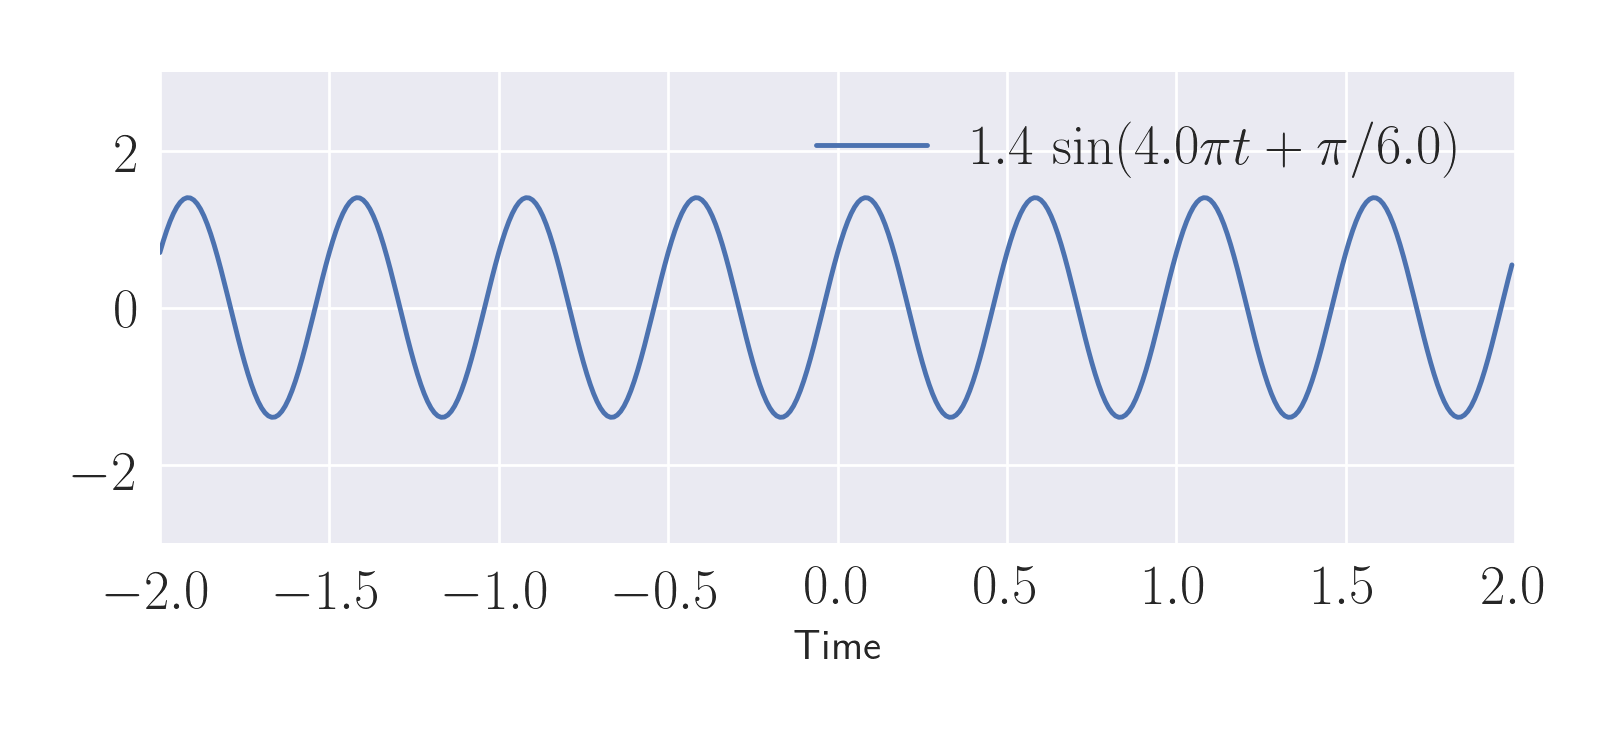
\includegraphics[width=\textwidth]{figs/ch2-sine.png}
% \caption{Continuous-time real exponential signals -- growing exponential on the left and a decaying exponential on the right.} ch2-\label{fig:ch2_sine}
% \end{figure}

% \begin{problem*}[frametitle=Discrete-time exponential signals]
%     Please verify that $T$ is the fundamental period of $x\ct{t} = A\sin\ct{\omega t + \phi}$.
% \end{problem*}

% The exponential signal was earlier introduced as the real exponential, as the parameters of the signal are real numbers. In fact a more general form of exponential singals is the complex exponential, where the parameters are allowed to be complex numbers. A complex exponential can be witten as,
% \[ x\left(t\right) = Ae^{bt}, \, t \in \mathbb{R}, \,\, A, b \in \mathbb{C} \]

% Consider a complex exponential signal $e^{j\omega t}$. This can written as the following using the \textit{Euler identity}.
% \[ e^{j\omega t} = \cos\left(\omega t\right) + j\sin\left(\omega t\right) \]

% Thus a continuous-time sinusoid can be written as the real or imaginary part of the complex exponential.
% \[ \cos\left(\omega t + \phi\right) = \Re\left(e^{j\omega t + \phi}\right) \]
% \[ \sin\left(\omega t + \phi\right) = \Im\left(e^{j\omega t + \phi}\right) \]

% Another representation of sinusoidal signals in terms of complex exponential is the following,
% \[ \cos\left(\omega t + \phi\right) = \frac{e^{\left(j\omega t + \phi\right)} + e^{-\left(j\omega t + \phi\right)}}{2} \]
% \[ \sin\left(\omega t + \phi\right) = \frac{e^{\left(j\omega t + \phi\right)} - e^{-\left(j\omega t + \phi\right)}}{2j} \]

% \subsection{Discrete-time sinusoids}
% The discrete-time equivalent of the sinusoids are represented as the following,
% \[ x\dt{n} = A \sin \ct{\Omega n + \phi} \]
% \noindent where, $A$ is the amplitude of the sinusoid, $\Omega$ is the discrete frequency (radians per sample), and $\phi$ is the phase. A plot of a discrete-time sinusoid is shown in Fig. \ref{fig:ch2-discsine}.
% \begin{figure}[h]
% \centering
%     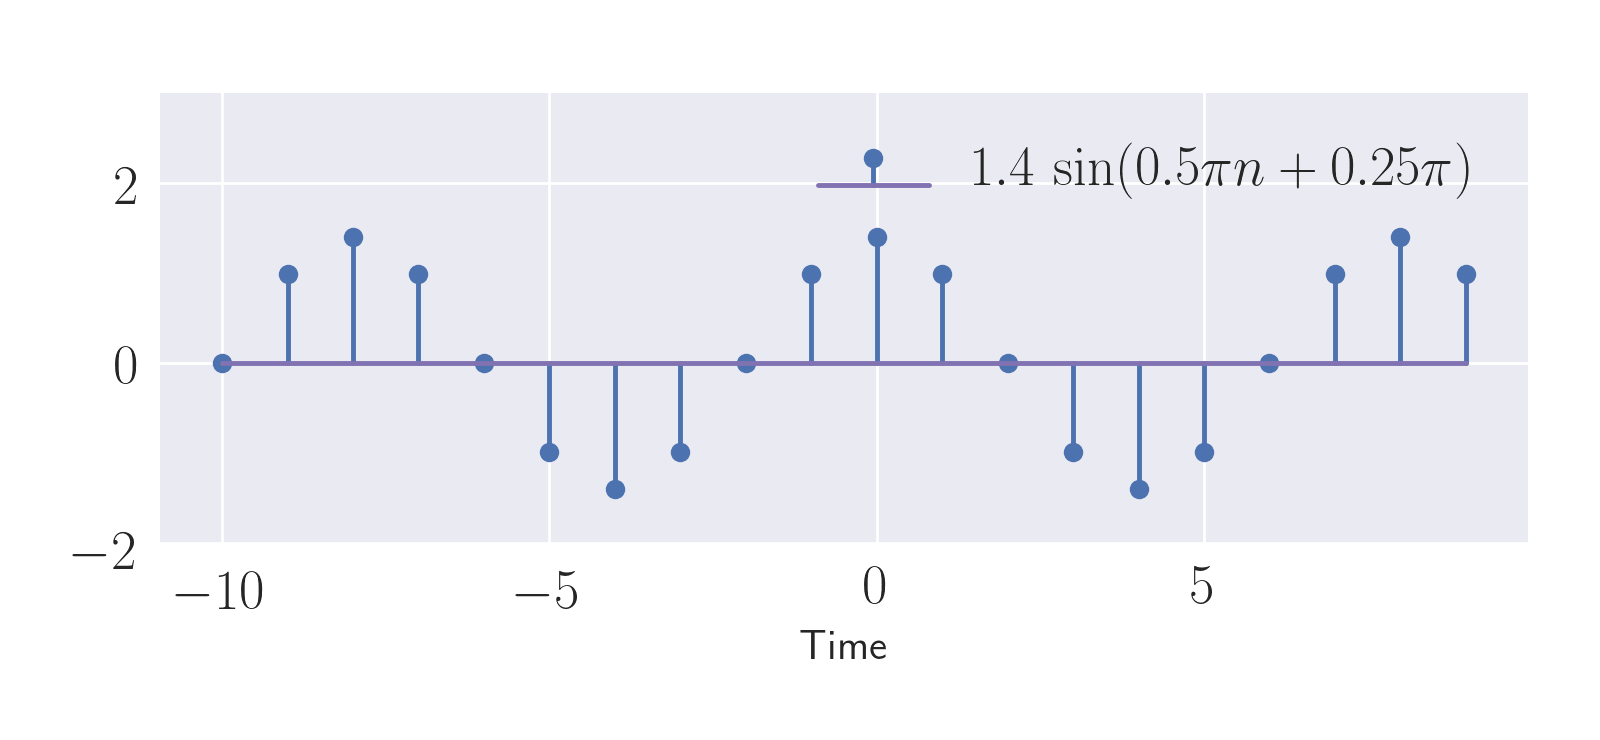
\includegraphics[width=\textwidth]{figs/ch2-discsine.png}
% \caption{Continuous-time real exponential signals -- growing exponential on the left and a decaying exponential on the right.} \label{fig:ch2-discsine}
% \end{figure}

% The period of $x\dt{n}$ is $N = k\frac{2\pi}{\Omega}$, where $k \in \mb{Z}$ such that $N \in \mb{Z}$. The discrete-time sinusoid has several features that are quite different to that of the continuous-time sinusoid. The following problems bring out some of these features.

% \begin{problem*}[frametitle=Discrete-time sinusoidal signals]
%     \begin{enumerate}
%         \item Please verify that $N = k\frac{2\pi}{\Omega}$ ($k \in \mb{Z}$ such that $N \in \mb{Z}$) is the period of $\sin \ct{\Omega n + \phi}$.
%         \item Prove that the discrete frequency $\Omega$ can only take values between $0 \leq \Omega < \pi$. 
%         \item There are some sinusoidal signals that are not periodic. Verify that $\sin \ct{n}$ is not periodic. 
%     \end{enumerate}
% \end{problem*}

% \section{Exponential Sinusoidal Signals}
% A natural extension of the representation of sinusoids in terms of complex exponentials is to combine the real and complex exponentials, which results in the exponential sinusoidal signals. A exponentially weighted sinusoid is obtained by multiplying a sinusoidal signal $\ct{\sin\ct{\omega t + \phi}}$ by a real exponential signal $\ct{e^{\alpha t}}$,
% \[ x\ct{t} = Ae^{\alpha t}\sin\ct{\omega t + \phi} \]

% \begin{figure}[h]
% \centering
%     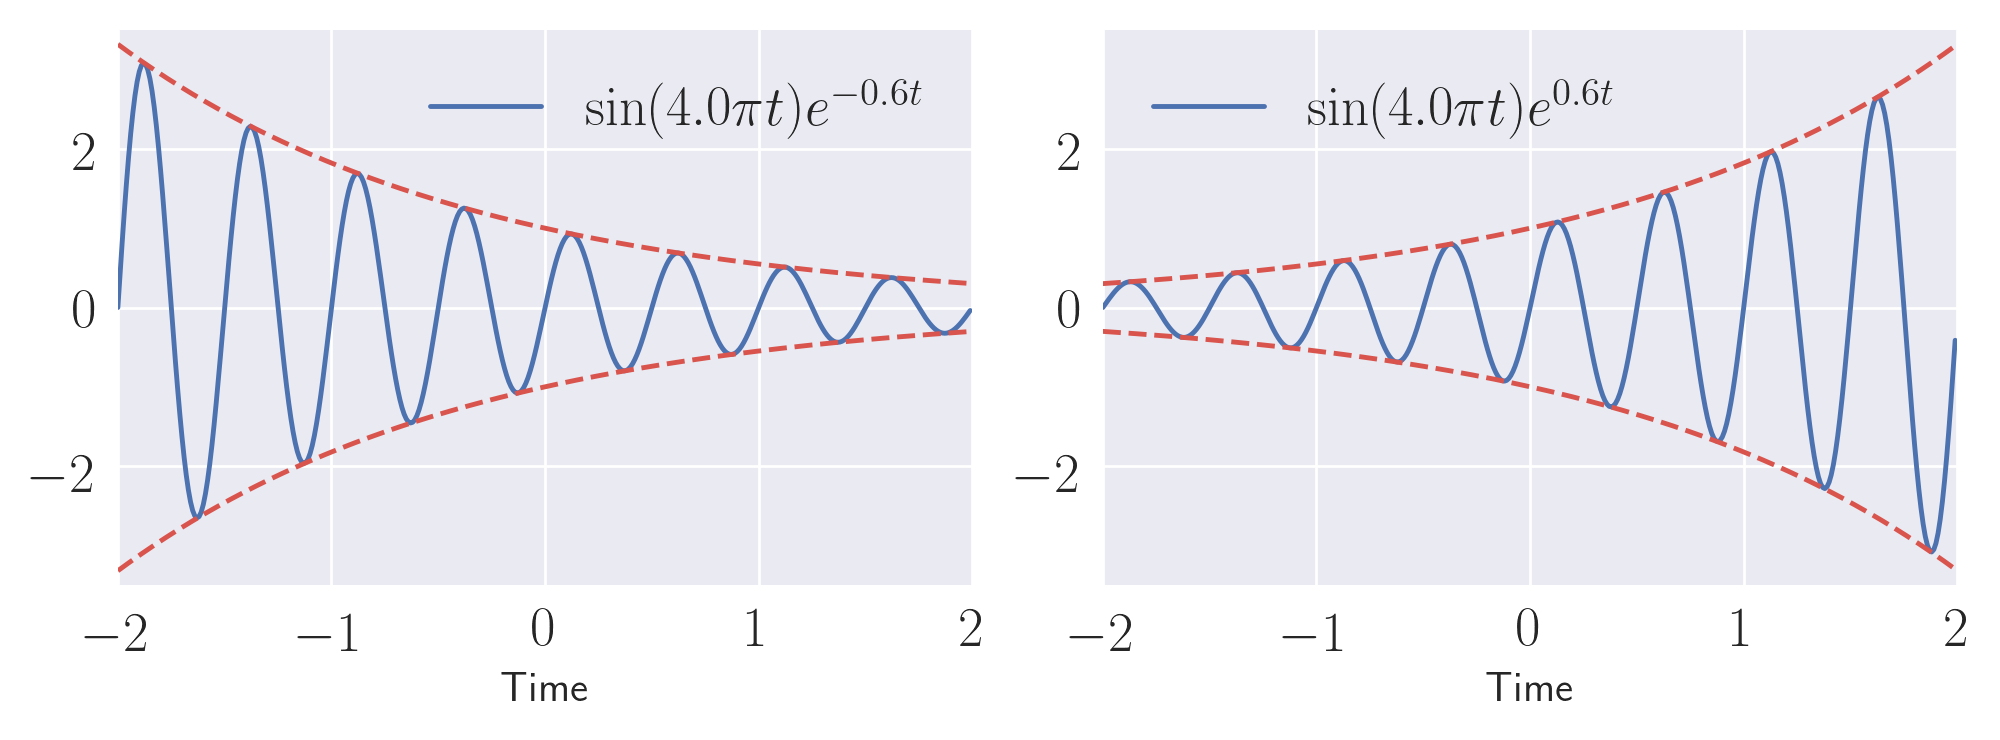
\includegraphics[width=\textwidth]{figs/ch2-expsine.png}
% \caption{Exponential continuous-time sinusoidal signals -- growing exponential on the left and a decaying exponential on the right.} \label{fig:ch2-expsine}
% \end{figure}

% \noindent $x\ct{t}$ can be represented using complex exponentials as,
% \[ x\ct{t} = Ae^{\alpha t}\sin\ct{\omega t + \phi} = A\frac{e^{\ct{\alpha + j\omega}t} - e^{-\ct{\alpha + j\omega}t}}{2j} = Ae^{\alpha t}\frac{e^{j\omega t} - e^{-j\omega t}}{2j} \]

% \begin{problem*}[frametitle=Discrete-time exponential sinusoidal signals]
%     Write down the expression for a discrete-time exponential sinusoidal signal. Explain how the different parameters affect the nature of the signal.
% \end{problem*}

% \section{Impulse function}
% \subsection{Continuous-time impulse function}
% The first and most important fact to remember about the impulse function is that it is not an ordinary function. The impulse function $\delta\left(t\right)$, also know as the Dirac delta function, is not characterized by the exact values it takes for the different values of its argument, rather it is characterized by the following property,
% \[ \int_{a}^{b}\delta\left(t\right)dt = 
% \begin{cases}
%     1, & 0 \in \left[a, b\right] \\
%     0, & \mathrm{Otherwise}
% \end{cases}
% \]

% This property tells us that the impulse function is concentrated around the origin $t = 0$. 

% A useful property of the impulse function is that \textit{\textbf{sifting property}}, For any ordinary function $f\left(t\right)$, which is continuous at $t = t_0$,
% \[ \int_{-\infty}^{\infty}f\left(t - t_0\right)\delta\left(t\right)dt = f\left(t_0\right) \]

% One way to think of the impulse function in terms of ordinary functions is to see it a limit of a sequence or family of functions. One sequence that is commonly encountered in books on signals and systems is the following,
% \[ g_{n}\left(t\right) = 
% \begin{cases}
% n, & -\frac{1}{2n} \leq t \leq \frac{1}{2n} \\
% 0, & \mathrm{Otherwise}
% \end{cases}
% \]

% This is a rectangular function that grows taller as $n \to \infty$. Now, lets take $g_{n}\left(t\right)$ and apply it on an ordinary function $f\ct{t}$,
% \[ \int_{-\infty}^{\infty}g_{n}\ct{t}f\ct{t}dt = \int_{-\frac{1}{2n}}^{\frac{1}{2n}}nf\ct{t}dt = f_n \]

% And,
% \[ \lim_{n\to\infty}\int_{-\infty}^{\infty}g_{n}\ct{t}f\ct{t}dt = \lim_{n\to\infty}f_n = f\ct{0} \]

% This is demonstrated in Fig. \ref{fig:ch2-impsifseq}.

% \begin{figure}[h]
% \centering
%     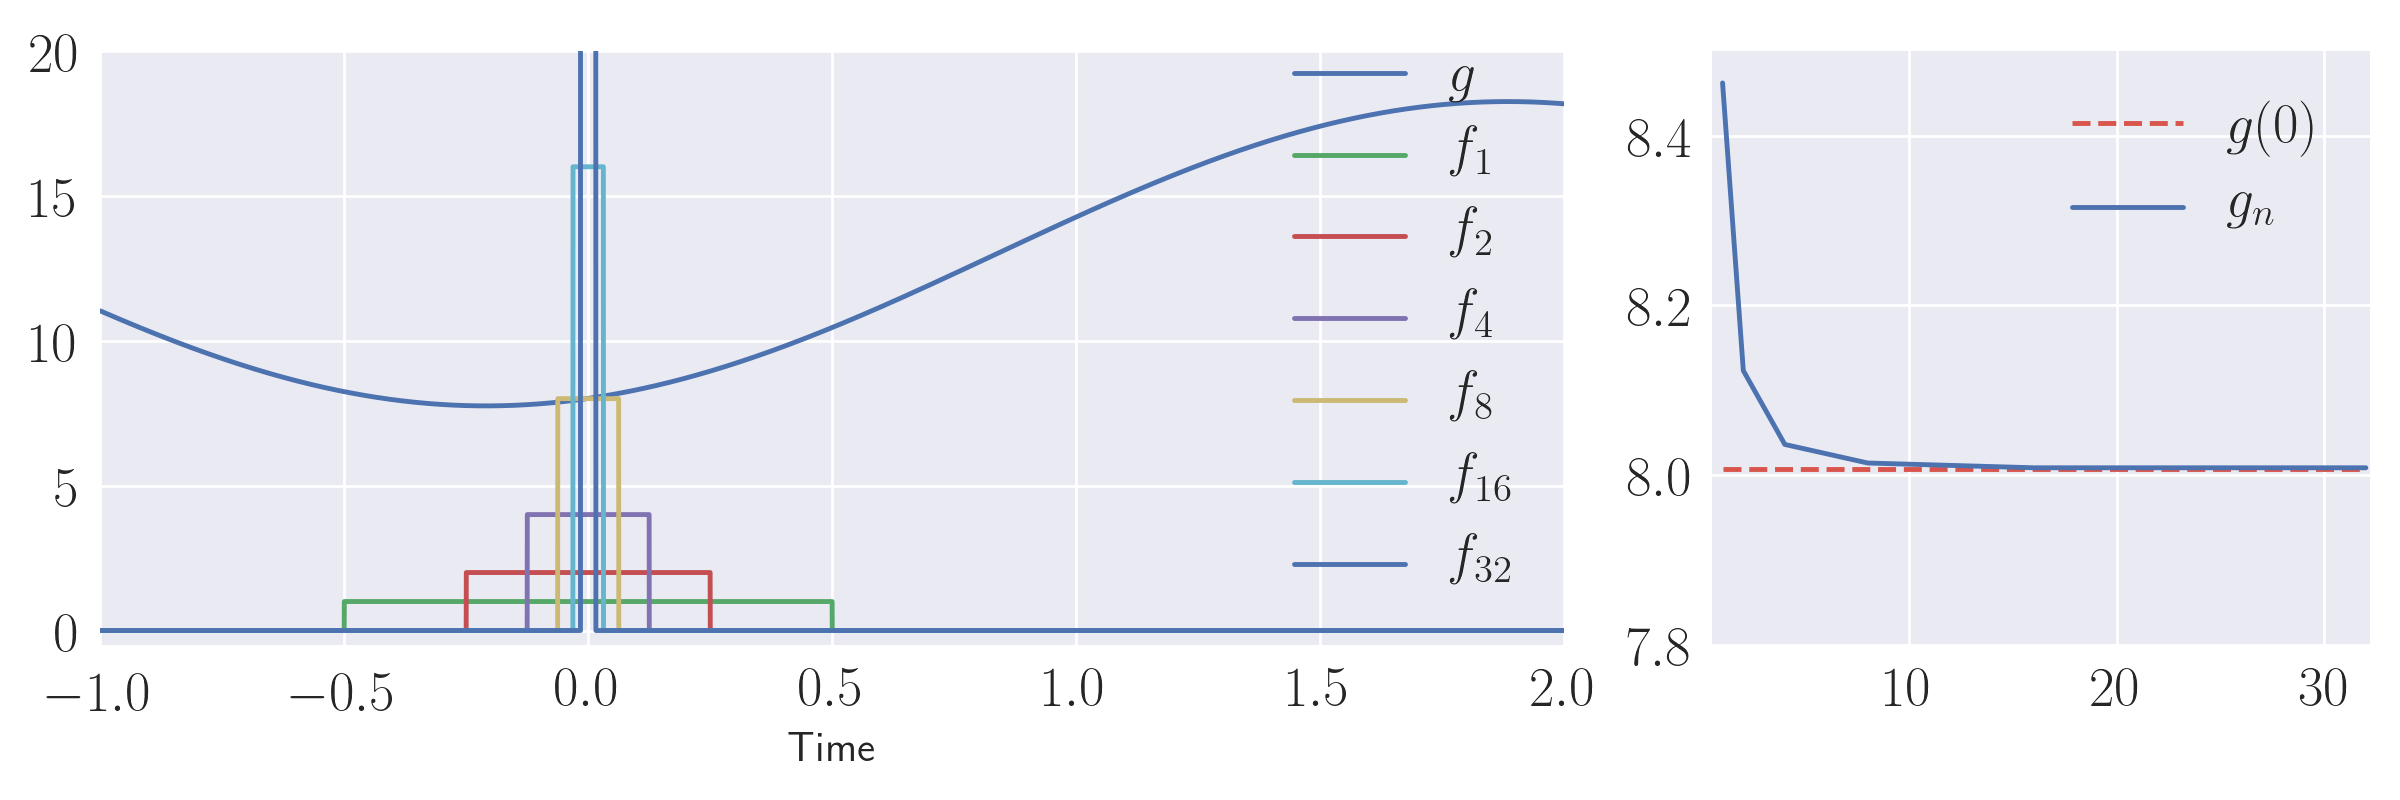
\includegraphics[width=\textwidth]{figs/ch2-impulsesift.png}
%     \caption{Viewing the impulse function as a limit of a sequence of rectangular pulses.}
%     \label{fig:ch2-impsifseq}
% \end{figure}

% \subsection{Discrete-time impulse function}
% The discrete-time impulse function is theoretically a much simpler function deal with. The discrete-time impulse function is defined as,
% \[ \delta\dt{n} = 
% \begin{cases}
%     1, & n = 0 \\
%     0, & n \neq 0
% \end{cases}
% \]

% \begin{figure}[h]
% \centering
%     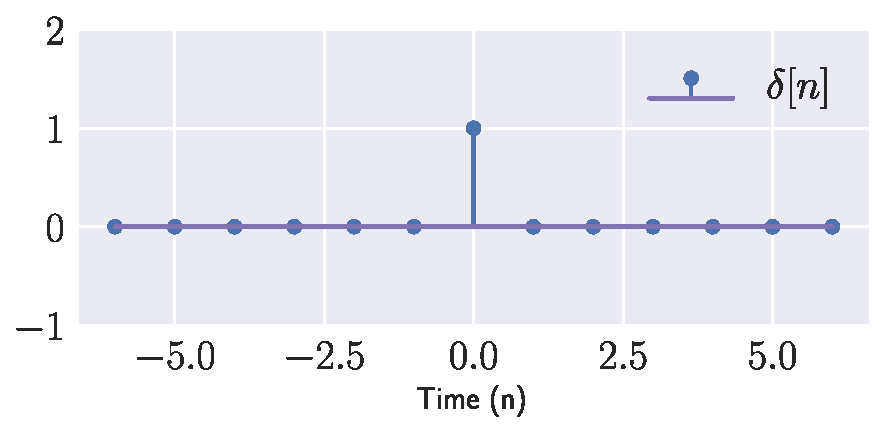
\includegraphics[width=0.65\textwidth]{figs/ch2-impulse-disc.eps}
%     \caption{Discrete-time impulse signal.}
%     \label{fig:ch2-impdisc}
% \end{figure}

% \subsection{Step Function}
% \subsection{Continuous-time step function}
% The step function is defined using the impulse function as the following,
% \[ 1\left(t\right) = \int_{-\infty}^{t}\delta\left(\tau\right)d\tau = 
% \begin{cases}
%     1, & t > 0 \\
%     0, & t < 0 \\
%     \frac{1}{2}, & t = 0
% \end{cases} 
% \]

% \noindent This function has a step discontinuity at $t = 0$.

% \begin{figure}[h]
% \centering
%     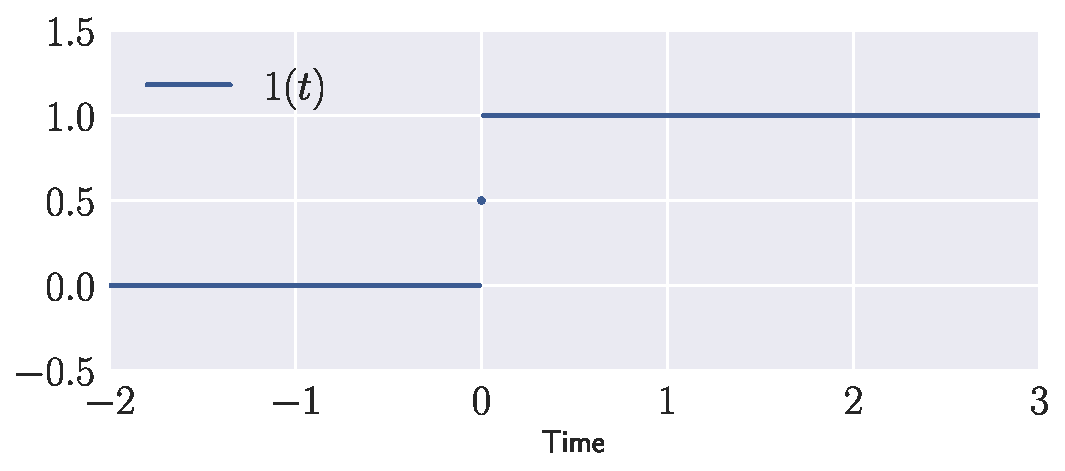
\includegraphics[width=0.7\textwidth]{figs/ch2-step-cont.eps}
%     \caption{Viewing the impulse function as a limit of a sequence of rectangular pulses.}
%     \label{fig:ch2-stepcont}
% \end{figure}

% \begin{problem*}[frametitle=Discrete-time step signal]
%     What would be definition of a discrete-time step function? How would you represent the discrete-time step function in terms of the discrete-time impulse function. 
% \end{problem*}